% A faire, fin de chapitre 4


\documentclass{report}
\usepackage{filecontents}

\usepackage[utf8]{inputenc}
\usepackage[T1]{fontenc}
\usepackage[francais]{babel}
\usepackage{listings}
\usepackage[a4paper]{geometry}
\usepackage{graphicx}
\usepackage[export]{adjustbox}
\usepackage{titlesec}
\usepackage{color}
\usepackage[toc, page]{appendix}
\usepackage{url}

\definecolor{xcodekw}{rgb}{0.75, 0.22, 0.60}
\definecolor{xcodestr}{rgb}{0.89, 0.27, 0.30}
\definecolor{xcodecmt}{rgb}{0.31, 0.73, 0.35}

\titleformat{\chapter}[display]
  {\centering\normalfont\huge\bfseries}
  {\chaptertitlename\ \thechapter}
  {20pt}
  {\Huge}

\geometry{hscale=0.75,vscale=0.85,centering}

\renewcommand{\thesection}{\arabic{section}}
\renewcommand\appendixtocname{Annexes}
\renewcommand\appendixname{Annexes}
\renewcommand\appendixpagename{Annexes}

\title{}
\author{Nicolas \bsc{Sias}, Youri \bsc{Mouton}, Samuel \bsc{Monroe}}

\date{30 Mai 2015}

\begin{document}

\maketitle

\newpage
\thispagestyle{empty}
\mbox{}

\tableofcontents

\chapter{Introduction}

	\section{Préambule}

		Ce rapport va présenter notre travail dans le cadre du cours de Traitement de Signal de 3e, sur le sujet de l'analyse d'un QR Code.\\

		Nous avons choisi de travailler à l'implémentation d'un Codeur-Décodeur de QR Code, ce en utilisant principalement les éléments offerts par MatLab, mais également en utilisant certains outils ou librairies lorsque des éléments de l'implémentation se révélaient trop techniques où ne pouvaient être accomplis sur base de nos connaissance ou du temps qui nous restait avant l'échéance.\\

		Nous allons commencer par exposer les détails d'une analyse sur le fonctionnement du QRCode en général, ainsi que sur la version avec laquelle nous avons choisi de travailler.\\
		Ensuite, un chapitre sera dédidé à la partie \textbf{décodeur} du code, suivi d'un chapitre sur le \textbf{codeur}.\\
		Nous terminerons par une conclusion, et une annexe sera présente et repertoriera notre bilbiographie ainsi que tout autre élément ayant servi à ce travail.\\

	\section{QR - Généralités}

		Le QR code est une sorte de code-barre en \textbf{2D}, il est formé d'une matrice de carrés noirs ou blancs dont la disposition définit le message contenu, et a été conçu par les Japonais de Denso-Wave pour permettre l'encodage de Kanji.\\

		Cette matrice est composée de séquences de positionnement ressemblants à trois carrés noirs content un plus petit carré noir également, le reste du contenu de la matrice représente l'information. Précisons nottamment que les versions plus évoluées possèdent aussi d'autres séquences dites d'alignement. \\
		Ces QR sont classifiés en versions qui précisent principalement la taille de la matrice.\\

		Un point très intéressant à propos des QR Codes est l'inclusion d'une correction d'erreur, composée d'information redondante dans la matrice et qui permet son décodage jusqu'à un certain niveau de dégradation.\\
		Il y a quatres niveaux de correction d'erreur, qui définissent jusqu'à pourcentage la matrice peut être dégradée et rester lisible par un décodeur : \\

		\begin{itemize}
			\item \textbf{L} : 7\%
			\item \textbf{M} : 15\%
			\item \textbf{Q} : 25\%
			\item \textbf{H} : 30\%\\
		\end{itemize}

		Enfin, comme laissé entendre précédemment, les QR peuvent représenter plusieurs types d'informations, et une séquence dans la matrice du code précisera le codage utilisé : \\

		\begin{itemize}
			\item \textbf{Numerique}
			\item \textbf{Alphanumérique}
			\item \textbf{Byte}
			\item \textbf{Kanji}\\
		\end{itemize}

	\section{QR - Version de travail et choix de modes}

		Pour des raisons de simplicité, nous avons décidé de se concentrer sur un seul type de code qui possèdera les caractéristiques suivantes : \\

		\begin{itemize}
			\item \textbf{Version} : 1, la matrice est donc de 21x21
			\item \textbf{Niveau EC} : H, la correction d'erreur se fera jusqu'à 30\% de dégradation du QR
			\item \textbf{Mode} : Byte
		\end{itemize}

\chapter{Décodeur de QRCode}

	\section{Détection et extraction du QR}

		Nous avons pour cette étape de détection et extraction, utilisé une application en C++ utilisant la librairie OpenCV.\\
		Cet extracteur se base sur l'utilisation d'une caméra et détecte dans le flux vidéo la présence du QRCode.\\

		Le choix d'utiliser une application tierce pour cette étape est déliberée, cette fonctionnalité nécéssite une connaissance très poussée de traitement de l'image ainsi que d'outils mathématiques et de la façon d'intégrer ceux-ci.\\

		Nous allons donc présenter et expliquer ici les différentes étapes qui mènent à la capture du Code.\\

		\subsection{Détection des marqueurs d'identification du QR Code}

			Voici un schéma précisant les éléments qui composent un QR Code de version 2 : \\

			\includegraphics[scale=0.3]{qr-code-parts.png}\\

			Cette première étape consiste, en l'utilisation de la fonctionnalité de détection de contours d'OpenCV.\\
			OpenCV identifie les contours présents dans une image, mais va également stocker la hierarchie entre ceux-ci, ce qui va permettre d'isoler le countour extérieur des marqueurs de placement au sein de l'image.\\

		\subsection{Détermination de l'indentité des marqueurs}

			Comme répété précédemment, un QR Code comprends trois marqueurs de positionnement, qu'OpenCV à détecter via détection de countours précédemment.\\

			Ces marqueurs sont nommés de la sorte : \\

			\begin{itemize}
				\item \textbf{TOP} : Celui dans le coin supérieur gauche
				\item \textbf{RIGHT} : Celui dans le coin supérieur droit
				\item \textbf{BOTTOM} : Celui dans le coin inférieur gauche\\
			\end{itemize}

			Leur identification est effectuée assez simplement. Le fait que ces marqueurs soient au nombre de trois, dans les coins d'un carré, permet d'utiliser un triangle rectangle.\\
			Celui-ci va être établi en utilisant les trois centres de masses établis par la détection de contours précédemment effectuée.\\
			Dès lors, l'hypothénuse permet d'identifier les points RIGHT et BOTTOM à ses extrémités, le point TOP étant en contact avec les deux côtés plus courts.\\

			La distinction entre BOTTOM et RIGHT se fait ensuite via placement de ce triangle dans un axe XY et en évaluant l'hypothénuse et de la droite passant par TOP et perpendiculaire à cet hypothénuse : \\

			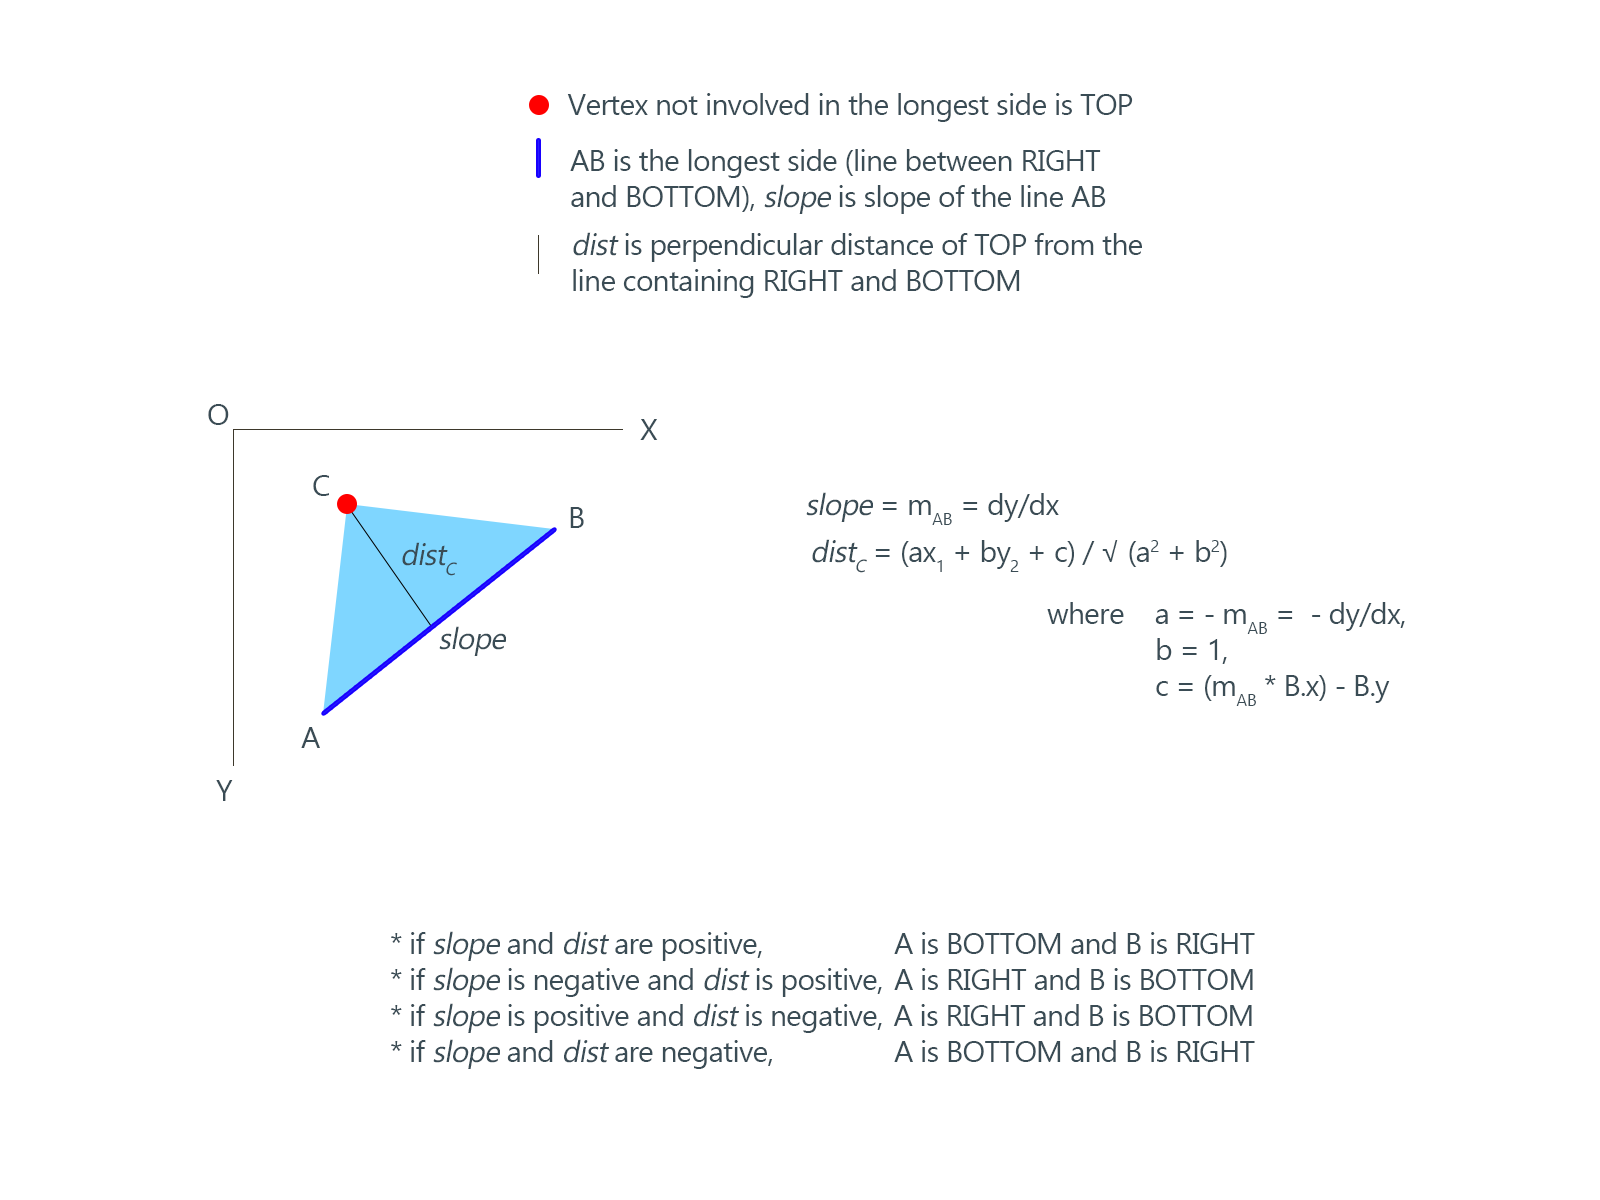
\includegraphics[scale=0.3]{align.png}

		\subsection{Identification des quatres coins des marqueurs de position}

			Cette opération est réalisée via la librairie OpenAR, elle est effectuée via l'utilisation des trois countours identifiées précédemment.\\
			Cette fonction retrouve les quatres coins des polygones et mesurant la distance de chaque point du périmètre par rapport au centre pour en identifier les points les plus éloignés.\\

		\subsection{Détermination des quatres points du QRCode}

			Une fois les quatres coins de chaque marqueur identifiés, il est aisé d'estimé les quatres coins du QRCode lui-même.\\

			Cette estimation est accomplie en étendant les lignes externes formées par BOTTOM et RIGHT, leur intersection crée le quatrième point N.\\

			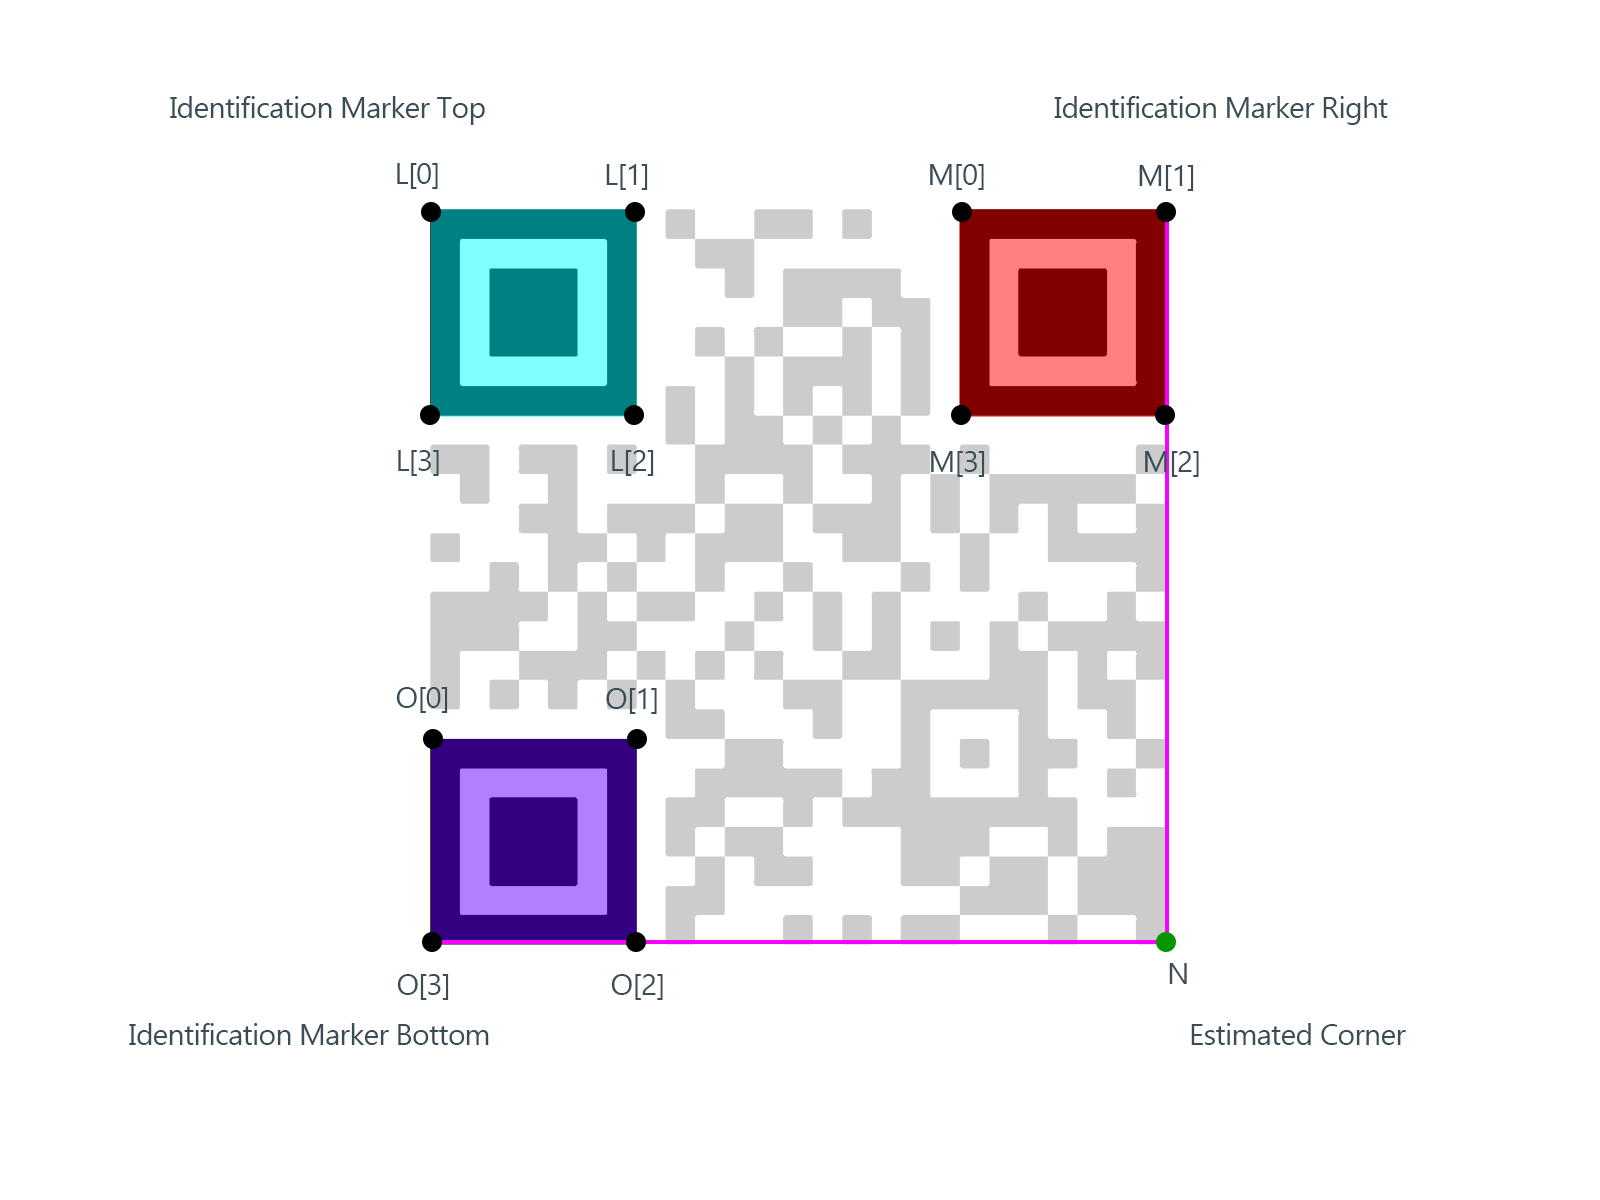
\includegraphics[scale=0.3]{naming.png}\\

		\subsection{Orientation du QRCode}

			Celle-ci est obtenue en utilisant la fonction \textbf{warpPerspective()} de OpenCV, pour rétablir le positionnement du QRCode en fonction de l'orientation du côté du triangle formé par TOP et RIGHT.\\

			\includegraphics[scale=0.3]{orient.png}\\

		\subsection{Traitement de l'image acquise dans MatLab}

			Une fois l'image du QRCode acquise via la méthode précédente, il reste à la traiter afin de pouvoir en retirer l'information contenue.\\

			L'image générée n'est pas forcément de la meilleure qualité qui soit, tout dépend des conditions dans lesquelles elle a été capturée, de la caméra utilisée, etc...\\

			\subsubsection{Ouverture de l'image}

				Celle-ci est réalisée via la commande : \textbf{qrcode = imread('qrcode.jpg')}

			\subsubsection{Transformation en image 2D de niveau de gris}

				Pour du traitement, il nous faut maintenant transformer cette image de QR Code en image de niveau de gris.\\

				Ceci est réalisé via la fonction \textbf{im2bw} qui va transformer une image en imagine binaire (composée de points noirs 0 ou blancs 1), sur base d'un niveau passé à cette même fonction.\\
				L'image retournée est donc une matrice \textbf{binaire}.\\

				Ceci est effectué via la commande : \textbf{qr = im2bw(qrcode, 0.5)}

			\subsubsection{Lissage}

				L'image présente des artefacts liés à sa capture, nous allons donc lui appliquer un filtre médian, plus adapté que le filtre linéaire, afin d'en réduire le bruit impulsionnel.\\

				\textbf{clean = medfilt2(qr)}

			\subsubsection{Redimensionnement de la matrice}

				Afin que l'information soit exploitable, ils nous faut revenir à la matrice d'origine de 21x21.\\
				Ceci va être accompli en créant une matrice de la taille voulue et en redimensionnant notre image filtrée avec celui-ci.\\

				\begin{itemize}
					\item \textbf{vector = [21 21]}
					\item \textbf{final = imresize(clean, vector)}
				\end{itemize}


		\subsection{Décodage de la matrice}


\chapter{Codeur de QRCode}
	
	Ce chapitre va s'attarder sur notre démarche portant sur le codeur d'un QR Code et son implémentation dans MatLab.\\
	Le résultat final voulu est l'obtention d'un code possédant les caractéristiques définies au début de ce rapport, uniquement en fournissant au programme une chaîne de caractère qui représentera le message à coder.\\

	Nous allons commencer par voir les spécifications de ce QRCode, et ensuite allons voir pas à pas comment ce QR est généré jusqu'à l'obtention du résultat final.\\

	Cette description des étapes sera volontairement résumée à l'essentiel, l'ensemble de notre code a été commenté, versionné et sera consultable via un lien vers le repository Github dans lequel il repose.\\

	\section{Préambule}

		Pour l'implémentation de notre solution, nous nous sommes basés sur un tutoriel du site Thonky destiné aux étudiants et conçu pour leur permettre d'implémenter leur propre codeur de Qr Code.\\
		Il explique de manière complète les différentes étapes du codage des données, de la génération du payload et des séquences de correction d'erreur.\\

	\section{Encodage des données}

		La séquence de bits de données utilisateur contient le mode = 0100 , mode byte sur 4 bits et le nombre de caractères du message est de maximum 7 pour ce QRv1 en mode byte.\\
		Notre message exemple est 'ephec', représenté par 00000101 sur 8 bits.\\

		On découpe ensuite notre message en couple de caractère et leur accordons une valeur selon la table ascii : 'ep' = 01000000, 'he' = 01010110, 'c' = 01010111', sur 8 bits.\\

		Il faut ensuite rajouter un terminateur de données de maximum quatres 0 si un byte n'est pas complété.\\

		L'étape finale est de rajouter une chaîne dite de \textbf{padding} jusqu'à ce que notre chaîne de données soit pleine, c'est-à-dire de 72bits pour une QRv1-h. Les spécifications QR indiquent la chaîne de padding suivante : \textbf{11101100 00010001}.\\

	\section{Encodage des erreurs}

		Cette étape de la génération du QR Code a été confiée au même site Thonky qui propose une interface de calcul des séquences d'erreurs, accédée via un Shell Script utilisant Curl et confiant nos bytes de data en base 10, récupérant ensuite l'output du site.\\

		Les séquences de calculs sont relativement complexes et surtout fastidieuses à implémenter, voici néanmoins un aperçu des outils mathématiques utilisé pour cette génération des codes correcteurs.\\

		\subsection{Reed-Solomon et la division polynomiale}

			Ces codes de correction d'erreurs sont générés en utilisant la méthode appelée Erreur de correction de Reed-Solomon, une partie de ce processus consiste en une division longue polynomiale, donc une division d'un polynome par un autre.\\

		\subsection{Groupe de Galois}

			Reed-Solomon utilise également une méthode appelée le groupe de Galois, qui est essentiellement un ensemble réduit de nombres, sur lesquels un nombre d'opérations mathématiques qui créeront des nombres déjà présent dans cet ensemble.\\

		\subsection{Blocs de corrections d'erreurs}

			Cette succession d'opérations sur les blocs de data vont mener sur la création de 17 blocs de correction d'erreur.\\

	\section{Génération du Qr Code}

		Pour générer le Qr Code une fois les blocs obtenus, il va falloir effectuer le placement des blocs dans la matrice, ainsi que les marqueurs de positionnement.\\

		La structure globale d'un QRCode v1 ainsi que le positionnement des différents blocs est le suivant : \\

		\includegraphics[scale=0.3]{bytes-disposition.png}\\

		Notre programme utilise trois scripts MatLab qui vont successivement placer les marqueurs de positionnement, les séquences de timing, ainsi que les données.\\

		\subsection{Exportation du résultat final}

			Une fois la matrice crée via le script MatLab, on dispose donc d'une matrice binaire de 21x21 prête à l'utilisation.\\

			Un simple \textbf{imshow()} permet d'observer le résultat.\\

\chapter{Conclusion}

	\section{Pistes d'améliorations}

		Une possible amélioration majeure que nous pourrions ajouter à notre projet, est un traitement d'une image afin de retrouver le QR Code dans elle-ci, traitement qui aurait été programmé par nos soins.\\
		De même pour un traitement et capture du QRCode dans une vidéo, étant donné que nous utilisons actuellement un programme tiers pour cette capture.\\

		Une autre possibilité d'amélioration serait une prise en charge de différentes versions de QR Code, ainsi que différents niveaux de correction d'erreurs et différents encodages.\\

	\section{FeedBack Personnels}

		\subsection{Youri Mouton}

		\subsection{Jonathan Seynaeve}

		\subsection{Samuel Monroe}

			Sur ce projet, j'ai surtout travaillé quant à la partie acquisition du QRCode, traitement de l'image obtenue afin de la transformer en matrice utilisable pour le décodage, ainsi qu'à la rédaction du rapport et du support de présentation du projet.\\

			J'aurais aimé créer une solution originale de capture du QRCode, soit via processing d'une image, soit via processing d'une vidéo.\\
			Néanmois, je suis satisfait du travail accompli par l'ensemble du groupe, et que nous ayons parcouru de manière relativement complète ce travail d'analyse du QR Code.\\

		\subsection{Nicolas Sias}

	\section{Conclusion}

	Ce projet a été une bonne expérience et nous a permis de progresser de manière générale dans le cours, nous avons également pu nous rendre compte de la complexité qui peut se cacher derrière un simple code QR, des outils mathématiques qui interviennent dans la génération et le décodage de celui-ci, ainsi que des diverses opérations utiles pour détecter un code dans une image.\\

\chapter{Bibliographie}

	\begin{itemize}
		\item Thonky - Génération de QR Code - \textbf{http://www.thonky.com/qr-code-tutorial/}
		\item OpenCV - Capture de QrCode - \textbf{http://dsynflo.blogspot.in/2014/10/opencv-qr-code-detection-and-extraction.html}
		\item Groupe de Galois - \textbf{https://fr.wikipedia.org/wiki/Groupe\_de\_Galois}
		\item QRCode - \textbf{http://www-igm.univ-mlv.fr/~dr/XPOSE2011/QRCode/index.html#1}
		\item Repository Github - \textbf{https://github.com/yrmt/qr}
	\end{itemize}

\end{document}